\clearpage
\section{Hasil Implementasi Perangkat Lunak}

\subsection{Implementasi Antarmuka}

Antarmuka JajanRia dibangun memakai Laravel Blade, JavaScript, dan templat baku \textit{AdminLTE}~3 dengan warna identitas hijau \texttt{\#2E8B3D}. Seluruh formulir, navigasi tab, dan interaksi laci mengambang menjaga posisi halaman agar pengguna tetap berada di konteks aksinya.

\subsubsection{Halaman Beranda dan Katalog Utama}
Halaman beranda publik menampilkan etalase kuliner sekitar Politeknik Negeri Batam (\textit{Kantin Gedung Utama}, \textit{Gerbang Utama}, \textit{Tower A}, \textit{Ruko KDA}, \textit{Halte Kampus}, dan \textit{Pujasera}). Di bagian atas tersedia bilah pencarian serta penyaring kategori, rentang harga, dan area kampus. Bagian utama memuat karosel lapak berperingkat tertinggi beserta tombol ``Bantuan'' menuju \textit{Customer Support} sebagaimana terlihat pada Gambar~\ref{fig:ui-landing}.

\begin{figure}[htbp]
\centering
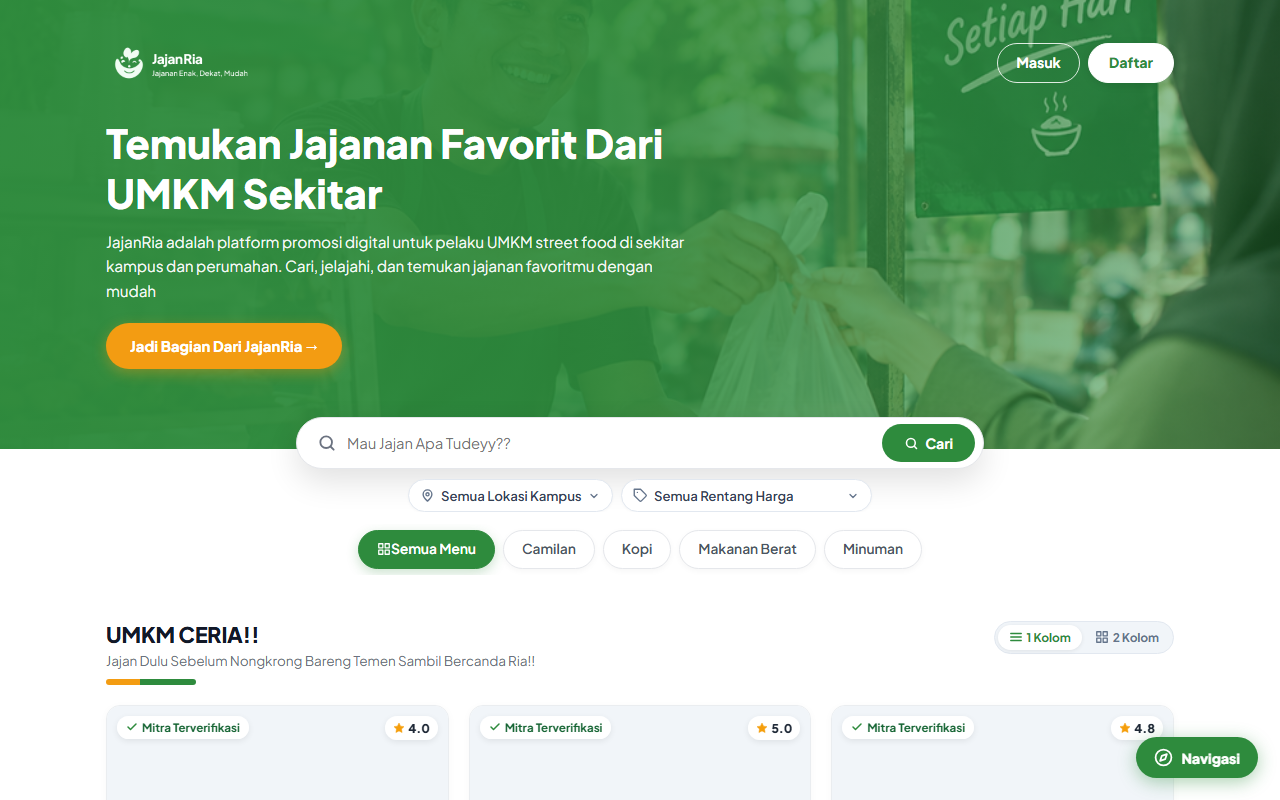
\includegraphics[width=0.92\textwidth]{assets/screens/01_landing.png}
\caption{Implementasi Halaman Beranda dan Katalog Utama}
\label{fig:ui-landing}
\end{figure}

\subsubsection{Halaman Masuk dan Pendaftaran Mitra Penjual}
Halaman masuk memfasilitasi autentikasi Pengunjung melalui \textit{Google Sign-In} (\textit{Firebase}) maupun tombol masuk dengan surel serta kata sandi untuk Penjual dan Admin. Sementara itu, halaman pendaftaran mitra menyediakan formulir tervalidasi dengan bidang nama pemilik, nama usaha, kontak, area, lokasi, unggah foto lapak, serta kata sandi. Kedua antarmuka tersebut ditunjukkan pada Gambar~\ref{fig:ui-auth}.

\begin{figure}[htbp]
\centering
\begin{minipage}[t]{0.48\textwidth}
  \centering
  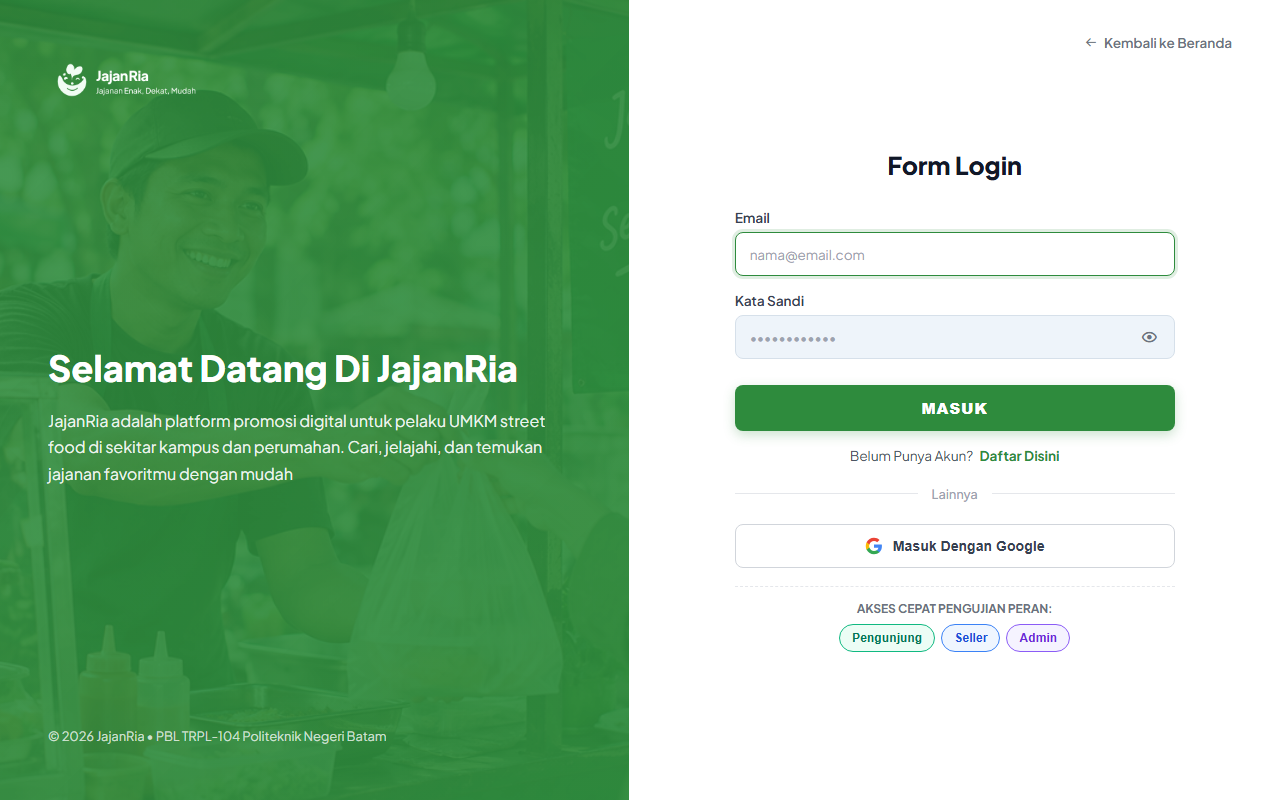
\includegraphics[width=\textwidth]{assets/screens/02_login.png}
  \par\small (a) Halaman Masuk
\end{minipage}\hfill
\begin{minipage}[t]{0.48\textwidth}
  \centering
  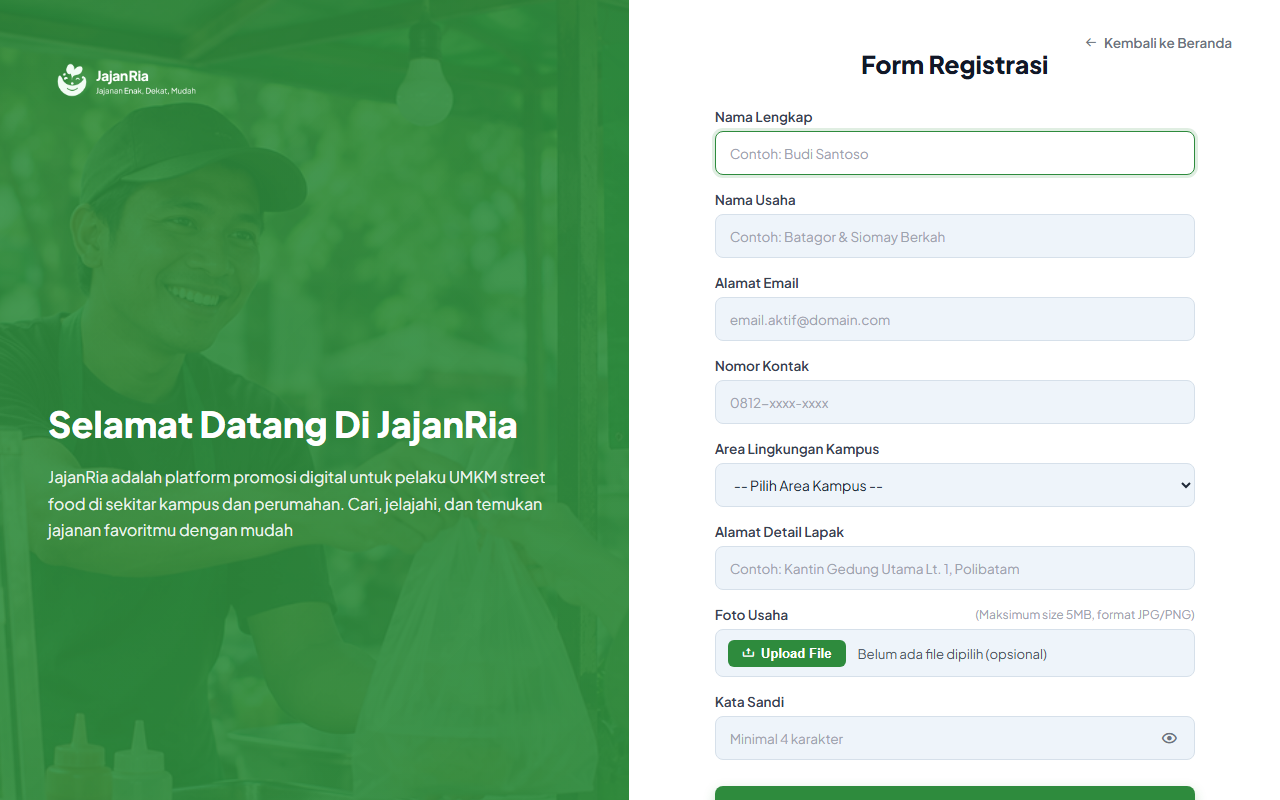
\includegraphics[width=\textwidth]{assets/screens/03_register.png}
  \par\small (b) Halaman Pendaftaran Mitra
\end{minipage}
\caption{Implementasi Antarmuka Autentikasi dan Registrasi Mitra UMKM}
\label{fig:ui-auth}
\end{figure}

\subsubsection{Halaman Detail Lapak, Keranjang, dan Modal Checkout}
Halaman detail lapak menyajikan informasi usaha, kelompok menu per kategori berikut penanda status habis, ulasan pembeli, serta bilah keranjang mengambang. Saat tombol ``Checkout \& Pembayaran'' dipilih, sistem membuka modal ringkasan pesanan, informasi pembayaran lapak, kolom unggah foto bukti bayar, serta catatan pesanan sebagaimana tampak pada Gambar~\ref{fig:ui-checkout}.

\begin{figure}[htbp]
\centering
\begin{minipage}[t]{0.48\textwidth}
  \centering
  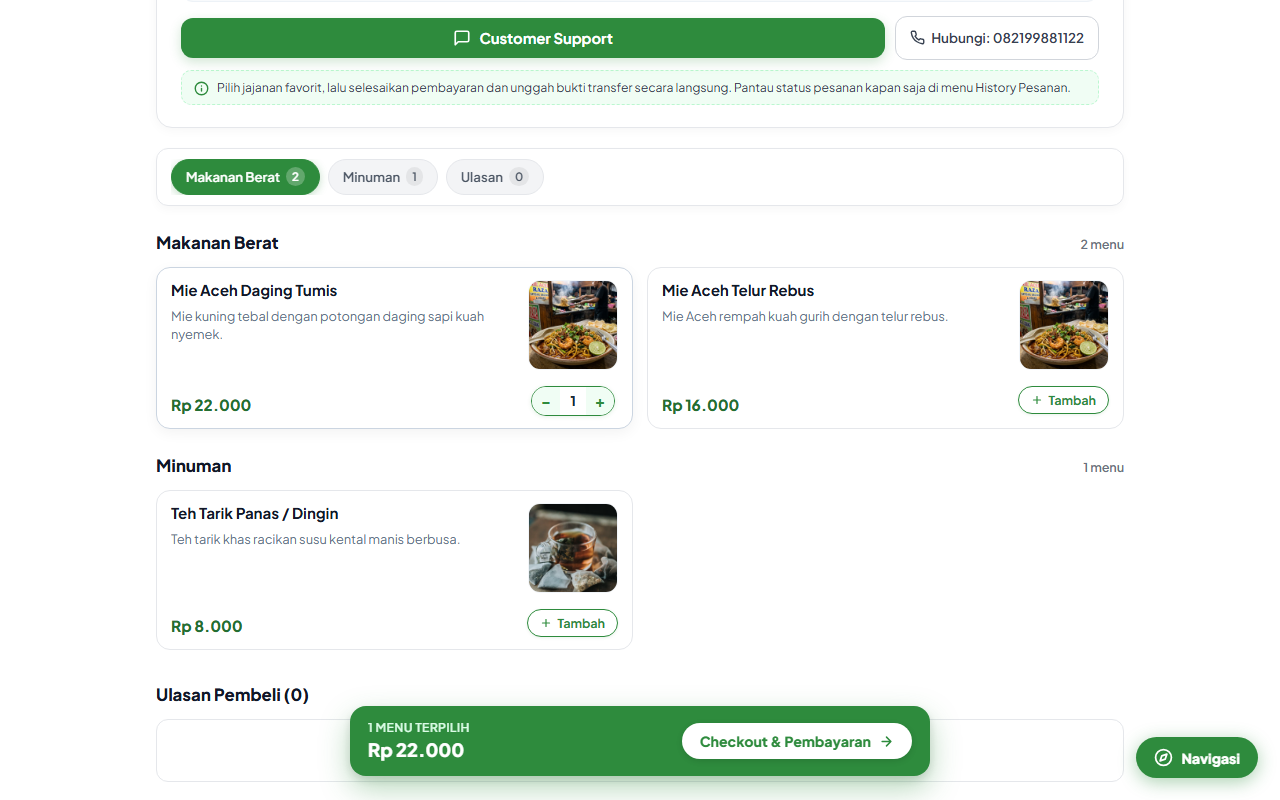
\includegraphics[width=\textwidth]{assets/screens/04_store_detail.png}
  \par\small (a) Detail Lapak \& Keranjang Belanja
\end{minipage}\hfill
\begin{minipage}[t]{0.48\textwidth}
  \centering
  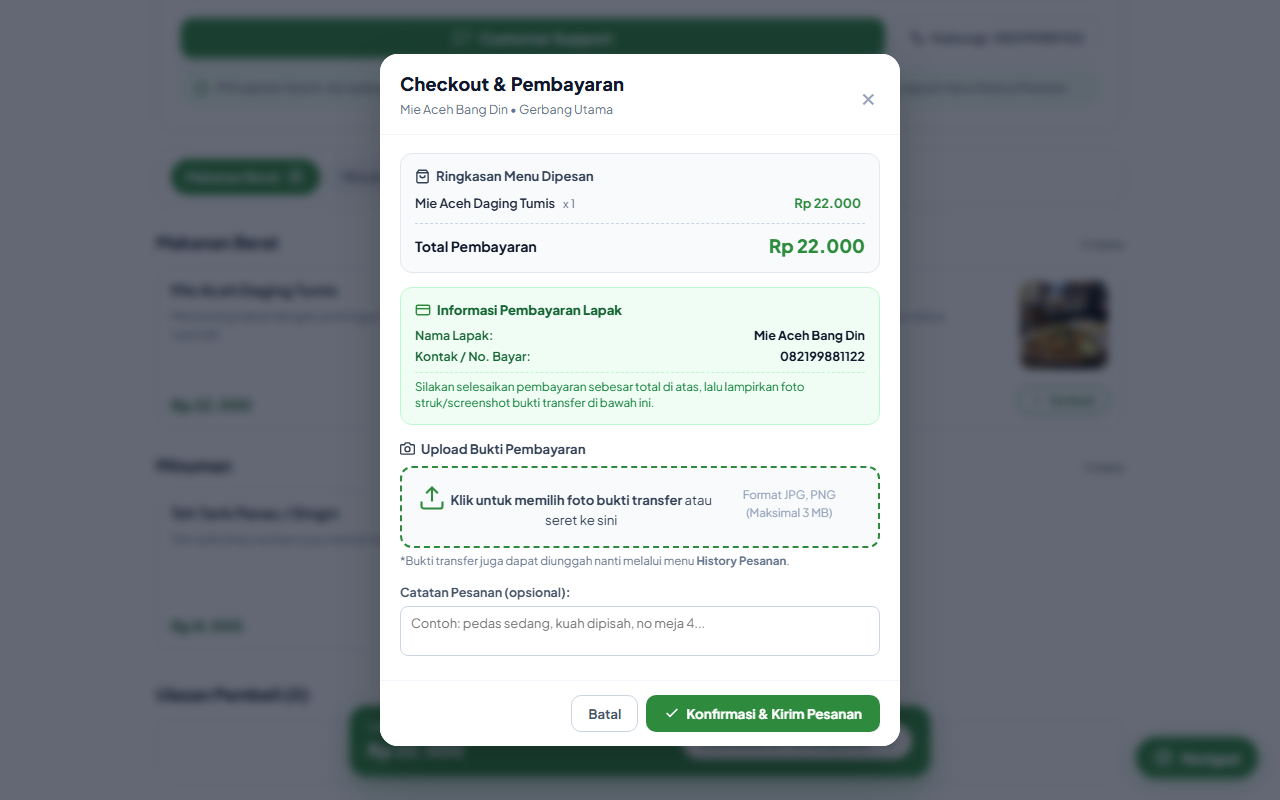
\includegraphics[width=\textwidth]{assets/screens/05_checkout_modal.png}
  \par\small (b) Modal \textit{Checkout} \& Pembayaran
\end{minipage}
\caption{Implementasi Detail Lapak UMKM dan Modal \textit{Checkout} Mandiri}
\label{fig:ui-checkout}
\end{figure}

\subsubsection{Laci History Pesanan dan Layanan Customer Support}
Pengunjung membuka menu peluncur \textit{Navigasi} di sudut kanan bawah untuk memantau transaksi pada laci \textit{History Pesanan}. Laci ini menampilkan status pesanan serta pembayaran, tombol unggah ulang bukti transfer, dan tombol ``Beri Penilaian'' saat pesanan berstatus \textit{selesai} dan \textit{lunas}. Saluran bantuan tersedia terpisah pada laci \textit{Customer Support} untuk berkirim pesan bersama Admin seperti pada Gambar~\ref{fig:ui-drawers}.

\begin{figure}[htbp]
\centering
\begin{minipage}[t]{0.48\textwidth}
  \centering
  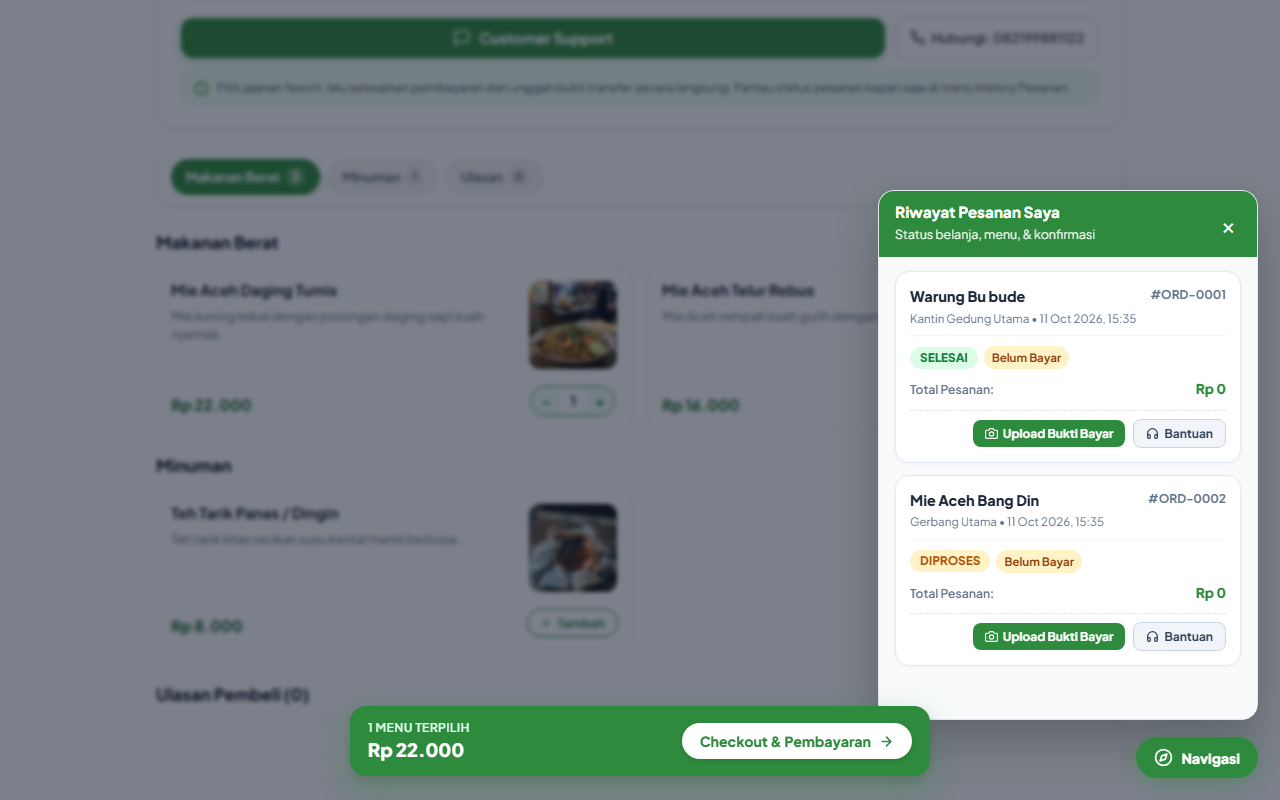
\includegraphics[width=\textwidth]{assets/screens/06_history_drawer.png}
  \par\small (a) Laci \textit{History Pesanan}
\end{minipage}\hfill
\begin{minipage}[t]{0.48\textwidth}
  \centering
  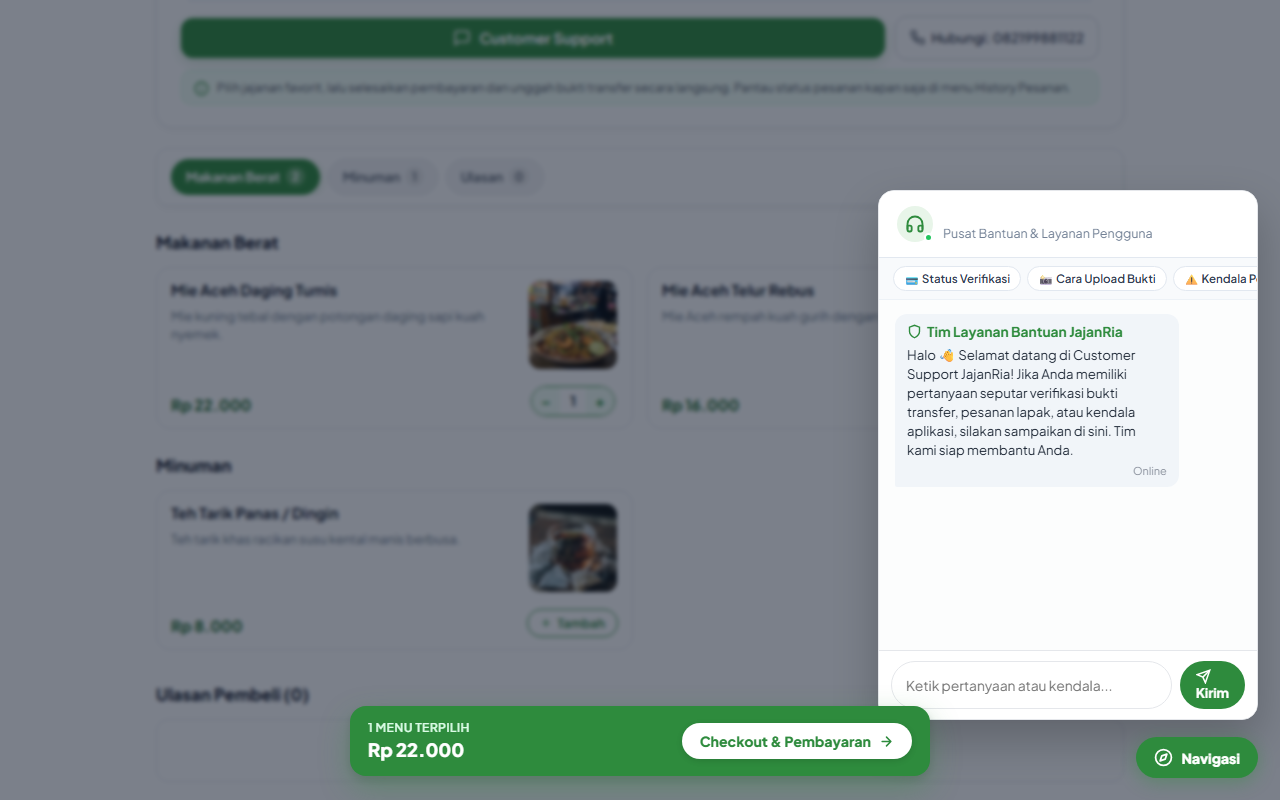
\includegraphics[width=\textwidth]{assets/screens/07_support_drawer.png}
  \par\small (b) Laci \textit{Customer Support}
\end{minipage}
\caption{Implementasi Laci \textit{History Pesanan} dan Pusat Bantuan Pelanggan}
\label{fig:ui-drawers}
\end{figure}

\subsubsection{Dasbor Penjual (Seller UMKM)}
Dasbor Penjual menyediakan lima tab fungsional yang menjaga posisi tab aktif setiap kali aksi dikirimkan, yaitu Ringkasan Toko, Kelola Menu \& Katalog, Pesan \& Pesanan, Profil Lapak UMKM, dan Rating \& Ulasan. Pada tab pesanan, rincian menu pesanan dan catatan pembeli tampil berdampingan, sedangkan tombol ``Selesai'' hanya aktif setelah Admin memverifikasi status pembayaran menjadi \textit{lunas}. Tampilan dasbor Penjual ditunjukkan pada Gambar~\ref{fig:ui-seller}.

\begin{figure}[htbp]
\centering
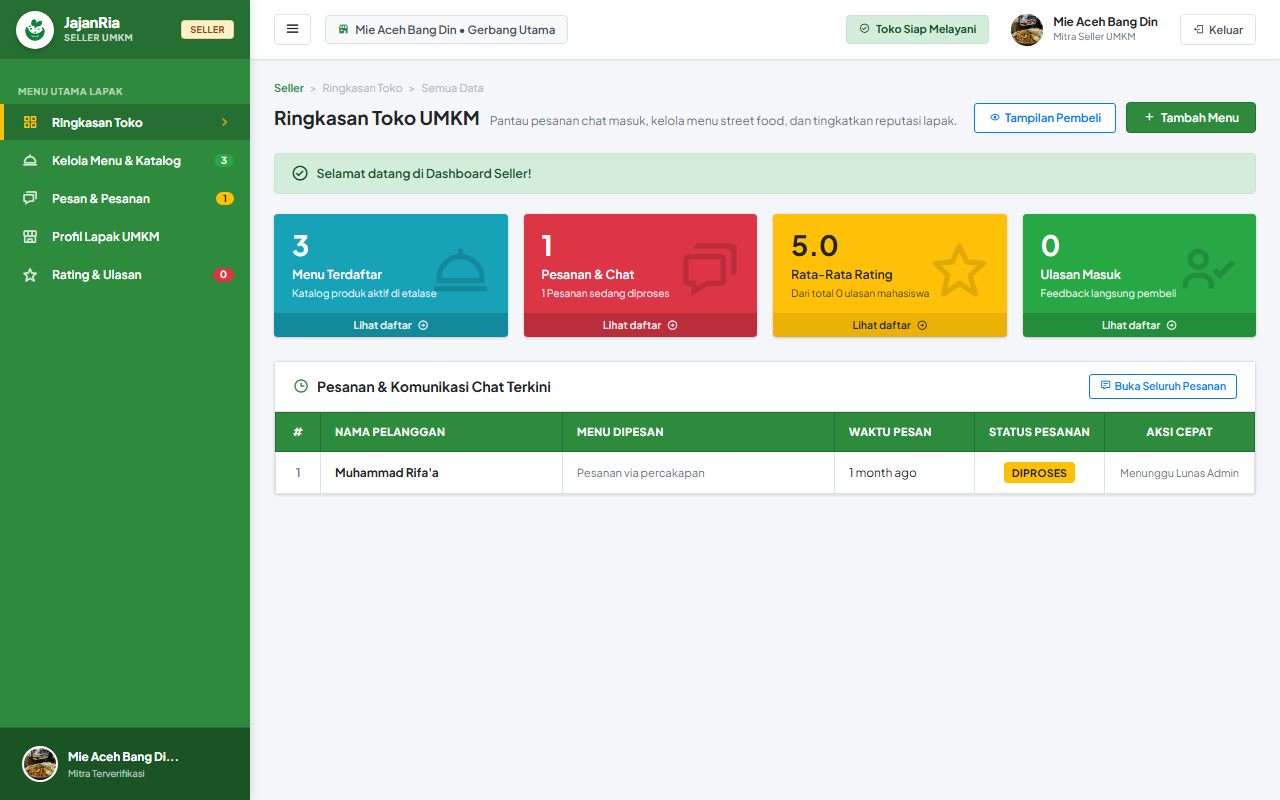
\includegraphics[width=0.90\textwidth]{assets/screens/08_seller_overview.png}
\par\vspace{0.2cm}\small (a) Tab Ringkasan Toko Penjual
\par\vspace{0.35cm}
\begin{minipage}[t]{0.48\textwidth}
  \centering
  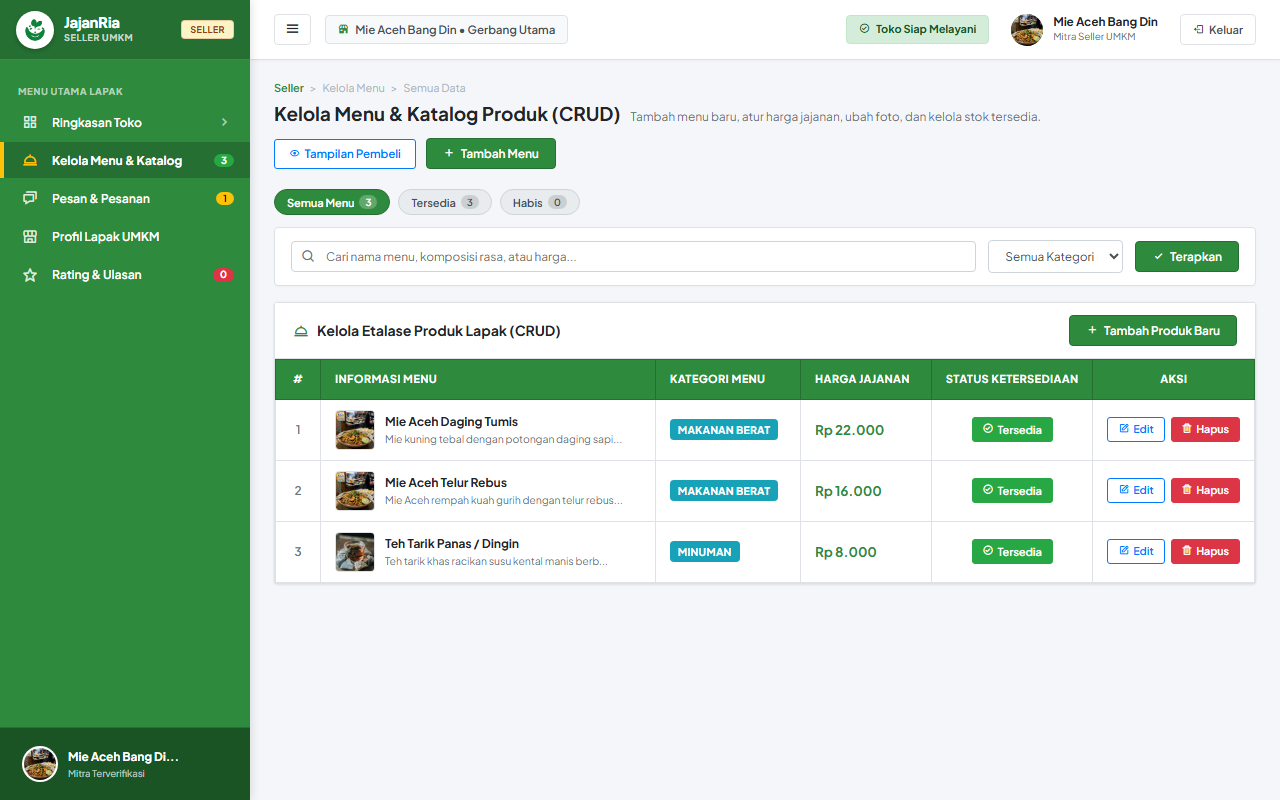
\includegraphics[width=\textwidth]{assets/screens/09_seller_products.png}
  \par\small (b) Tab Kelola Menu \& Ketersediaan
\end{minipage}\hfill
\begin{minipage}[t]{0.48\textwidth}
  \centering
  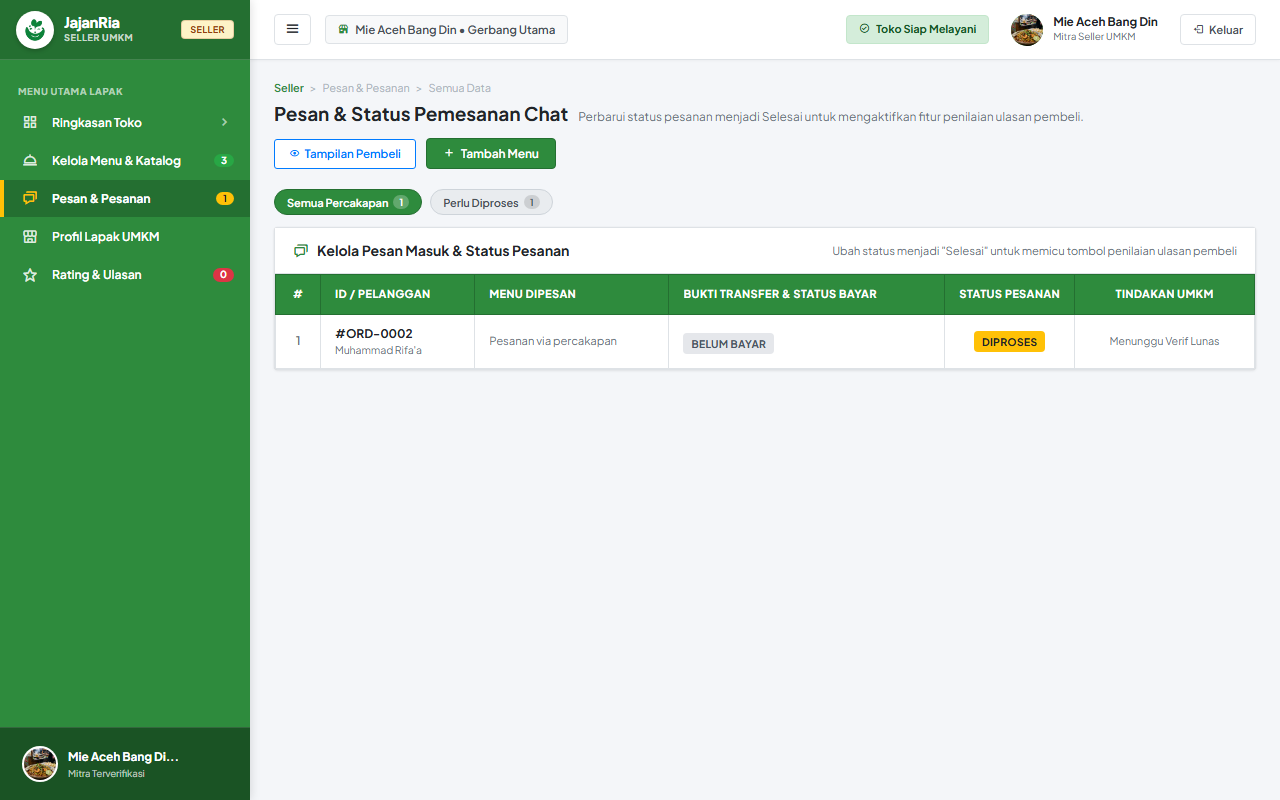
\includegraphics[width=\textwidth]{assets/screens/10_seller_orders.png}
  \par\small (c) Tab Daftar Pesanan \& Status Bayar
\end{minipage}
\caption{Implementasi Dasbor Operasional Penjual UMKM}
\label{fig:ui-seller}
\end{figure}

\subsubsection{Panel Administrator}
Panel Administrator menjadi pusat kendali platform dengan delapan tab terintegrasi: Monitoring \& Statistik, Verifikasi Seller Baru, Verifikasi Pembayaran, Kelola Mitra UMKM, Kelola Kategori Menu, Moderasi Ulasan, \textit{Customer Support}, dan Manajemen User. Seluruh tombol aksi kini bertahan pada tab aktif masing-masing, termasuk modal alasan penolakan bukti bayar dan proteksi hapus kategori berproduk aktif. Antarmuka panel Admin ditunjukkan pada Gambar~\ref{fig:ui-admin}.

\begin{figure}[htbp]
\centering
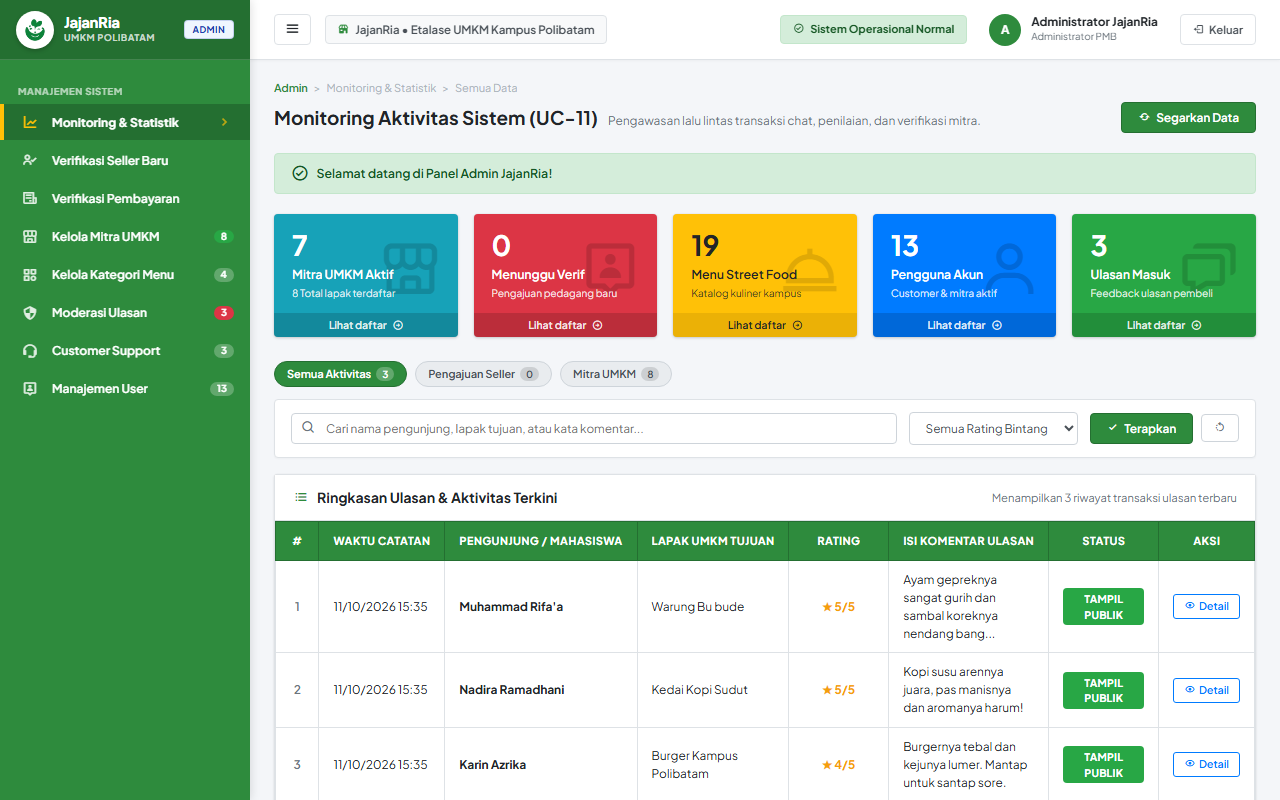
\includegraphics[width=0.90\textwidth]{assets/screens/11_admin_monitoring.png}
\par\vspace{0.2cm}\small (a) Tab Monitoring \& Statistik Platform
\par\vspace{0.35cm}
\begin{minipage}[t]{0.48\textwidth}
  \centering
  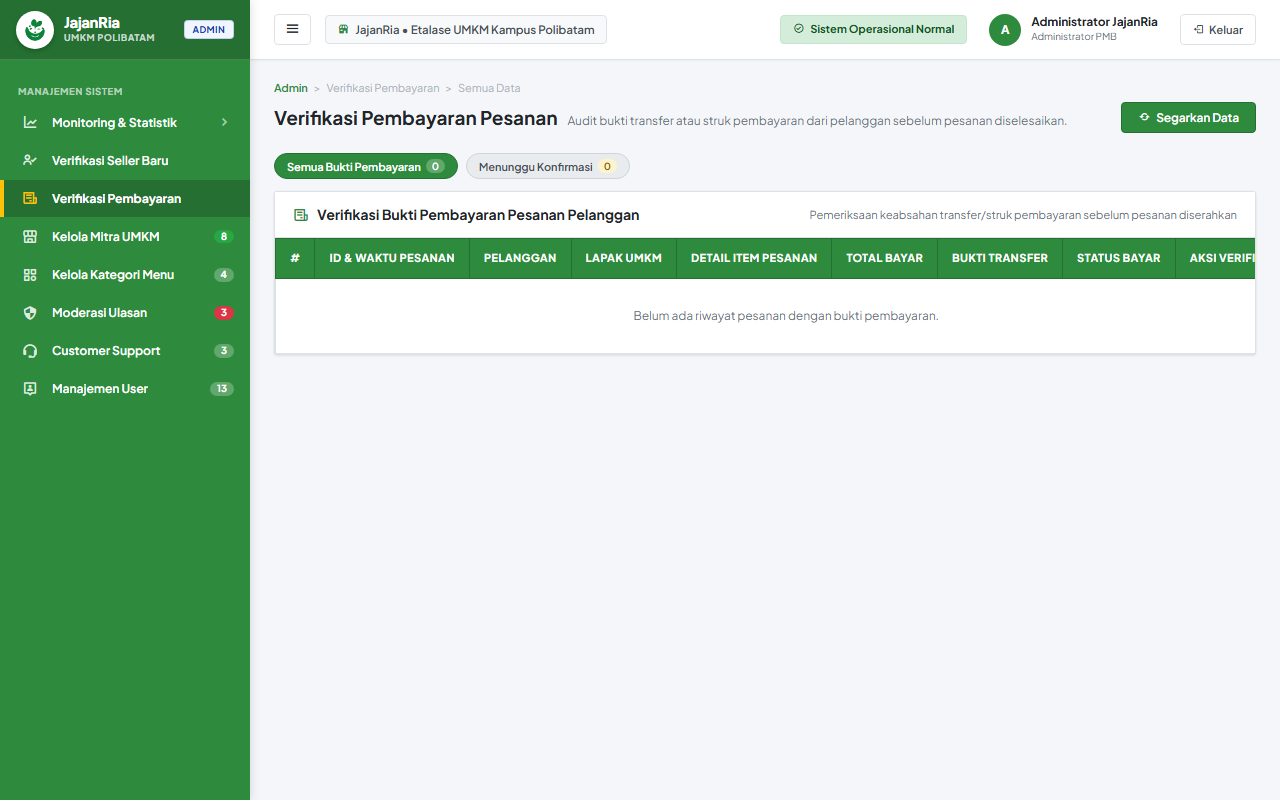
\includegraphics[width=\textwidth]{assets/screens/12_admin_payments.png}
  \par\small (b) Tab Verifikasi Pembayaran Manual
\end{minipage}\hfill
\begin{minipage}[t]{0.48\textwidth}
  \centering
  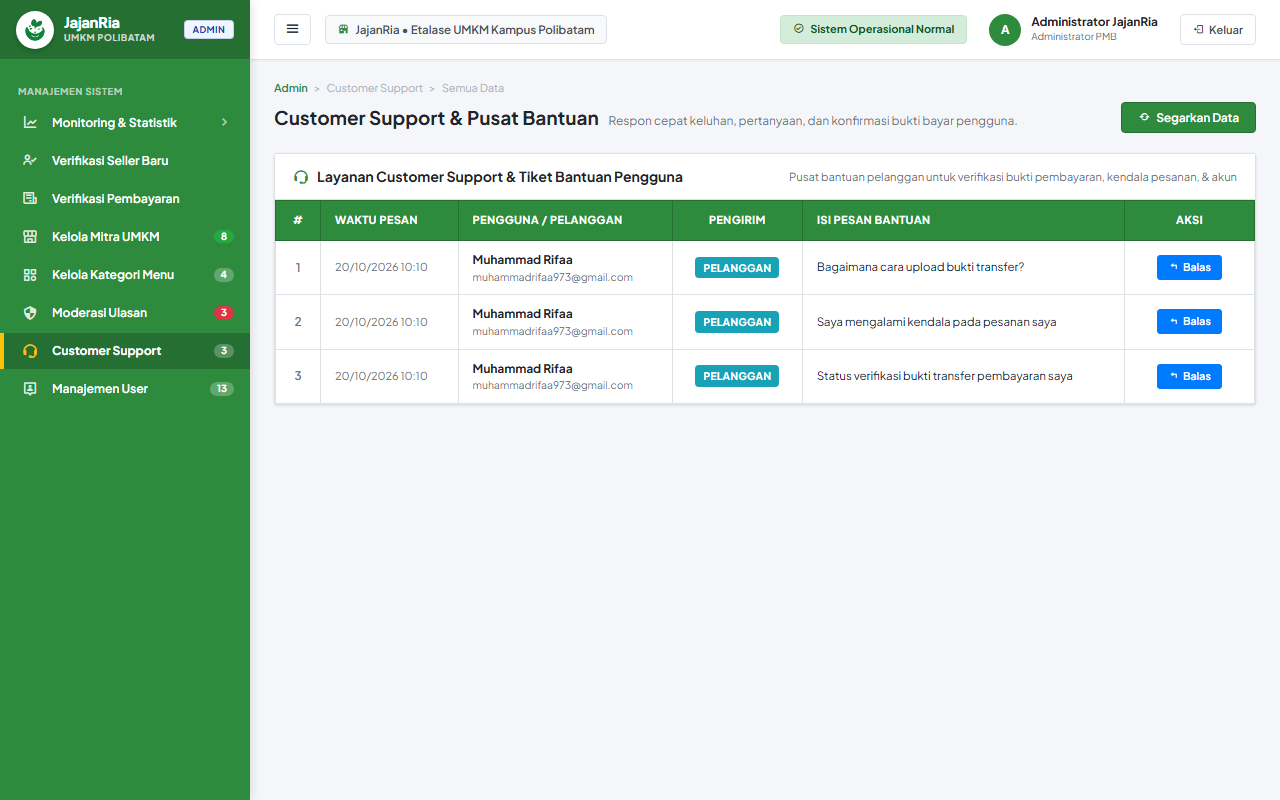
\includegraphics[width=\textwidth]{assets/screens/13_admin_support.png}
  \par\small (c) Tab Layanan \textit{Customer Support}
\end{minipage}
\caption{Implementasi Panel Administrator JajanRia}
\label{fig:ui-admin}
\end{figure}

\subsection{Implementasi Basis Data}

\subsubsection{Sistem Manajemen Basis Data dan Struktur Tabel}
Sistem JajanRia berjalan di atas sistem manajemen basis data relasional \textit{Structured Query Language} (SQL) MySQL versi \texttt{10.4.32-MariaDB} pada basis data \texttt{jajanria} dengan set karakter \texttt{utf8mb4\_unicode\_ci}. Skema basis data dibangun melalui 13 berkas migrasi Laravel~11 dan menghasilkan 16 tabel total. Tabel tersebut terdiri dari tujuh tabel domain aplikasi serta sembilan tabel kerangka kerja (\texttt{migrations}, \texttt{sessions}, \texttt{cache}, \texttt{cache\_locks}, \texttt{jobs}, \texttt{job\_batches}, \texttt{failed\_jobs}, \texttt{password\_\allowbreak reset\_tokens}, dan \texttt{users}). Inventaris tujuh tabel domain beserta volume baris aktual disajikan pada Tabel~\ref{tab:inventaris-db}.

\renewcommand{\arraystretch}{1.22}
\begin{longtable}{|L{2.8cm}|C{2.0cm}|L{\dimexpr\textwidth-2.8cm-2.0cm-6\tabcolsep-4\arrayrulewidth\relax}|}
\caption{Inventaris Tabel Domain Basis Data \texttt{jajanria}}
\label{tab:inventaris-db} \\
\hline
\rowcolor{TableHeadBg}
\textbf{Nama Tabel} & \textbf{Jumlah Baris} & \textbf{Fungsi Utama dalam Sistem} \\
\hline
\endfirsthead
\hline
\rowcolor{TableHeadBg}
\textbf{Nama Tabel} & \textbf{Jumlah Baris} & \textbf{Fungsi Utama dalam Sistem} \\
\hline
\endhead
\hline
\endfoot
\texttt{t\_user} & 13 & Akun Pengunjung, Penjual, dan Administrator berikut status verifikasi serta keaktifan. \\
\hline
\texttt{t\_umkm} & 8 & Profil lapak UMKM kuliner, lokasi rinci, kawasan area, kontak, dan foto lapak. \\
\hline
\texttt{t\_kategori} & 4 & Daftar kategori menu unik (\textit{Makanan Berat}, \textit{Camilan}, \textit{Minuman}, \textit{Kopi}). \\
\hline
\texttt{t\_produk} & 19 & Menu kuliner setiap UMKM beserta harga dan penanda ketersediaan (\texttt{tersedia}). \\
\hline
\texttt{t\_pesan} & 15 & Riwayat tiket \textit{Customer Support} (\texttt{id\_umkm = \textit{null}}) dan log pesan lama. \\
\hline
\texttt{t\_pesanan} & 7 & Transaksi pesanan langsung berisi \texttt{items\_detail}, catatan, bukti bayar, dan status. \\
\hline
\texttt{t\_ulasan} & 3 & Peringkat (1--5), komentar pembeli, balasan penjual, serta status moderasi. \\
\hline
\end{longtable}

\subsubsection{Contoh Data Aktual Basis Data}
Cuplikan isi nyata dari basis data \texttt{jajanria} untuk tabel pengguna, UMKM, kategori, produk, dan ulasan ditampilkan pada Tabel~\ref{tab:contoh-data-db}. Kolom kredensial seperti \textit{hash} kata sandi maupun pengenal internal Firebase tidak dicantumkan demi menjaga keamanan data.

\renewcommand{\arraystretch}{1.20}
\begin{longtable}{|L{2.2cm}|L{1.55cm}|L{\dimexpr\textwidth-2.2cm-1.55cm-6\tabcolsep-4\arrayrulewidth\relax}|}
\caption{Cuplikan Data Aktual pada Basis Data \texttt{jajanria}}
\label{tab:contoh-data-db} \\
\hline
\rowcolor{TableHeadBg}
\textbf{Tabel} & \textbf{ID Baris} & \textbf{Cuplikan Nilai Kolom Utama} \\
\hline
\endfirsthead
\hline
\rowcolor{TableHeadBg}
\textbf{Tabel} & \textbf{ID Baris} & \textbf{Cuplikan Nilai Kolom Utama} \\
\hline
\endhead
\hline
\endfoot
\texttt{t\_user} & \texttt{id=1} & \texttt{nama="Administrator JajanRia"}, \texttt{role="admin"}, \texttt{status\_verifikasi="terverifikasi"}, \texttt{is\_active=1} \\
\hline
\texttt{t\_user} & \texttt{id=6} & \texttt{nama="Pemilik Mie Aceh Bang Din"}, \texttt{role="seller"}, \texttt{status\_verifikasi="terverifikasi"}, \texttt{is\_active=1} \\
\hline
\texttt{t\_umkm} & \texttt{id=2} & \texttt{nama\_usaha="Mie Aceh Bang Din"}, \texttt{area="Gerbang Utama"}, \texttt{kontak="082199881122"} \\
\hline
\texttt{t\_umkm} & \texttt{id=4} & \texttt{nama\_usaha="Kedai Kopi Sudut"}, \texttt{area="Ruko KDA"}, \texttt{kontak="087733119002"} \\
\hline
\texttt{t\_kategori} & \texttt{id=1..4} & \texttt{Makanan Berat} (1), \texttt{Camilan} (2), \texttt{Minuman} (3), \texttt{Kopi} (4) \\
\hline
\texttt{t\_produk} & \texttt{id=5} & \texttt{id\_umkm=2}, \texttt{id\_kategori=1}, \texttt{nama\_produk="Mie Aceh Daging Tumis"}, \texttt{harga=22000.00}, \texttt{tersedia=1} \\
\hline
\texttt{t\_produk} & \texttt{id=7} & \texttt{id\_umkm=2}, \texttt{id\_kategori=3}, \texttt{nama\_produk="Teh Tarik Panas / Dingin"}, \texttt{harga=8000.00}, \texttt{tersedia=1} \\
\hline
\texttt{t\_ulasan} & \texttt{id=1} & \texttt{id\_pesanan=1}, \texttt{id\_umkm=1}, \texttt{rating=5}, \texttt{disembunyikan=0} \\
\hline
\end{longtable}

\subsubsection{Contoh Kueri yang Diimplementasikan}
Operasi akses data memakai pemetaan relasional objek (\textit{Object-Relational Mapping} atau ORM) Eloquent pada lapisan kontroler sehingga terlindung oleh pengikatan parameter untuk mencegah injeksi kueri SQL. Tiga kueri inti pada alur pencarian, transaksi \textit{checkout}, dan verifikasi pembayaran disajikan pada Kode~\ref{lst:kueri-app}.

\begin{lstlisting}[language=PHP, caption={Contoh Kueri Aplikasi pada Kontroler JajanRia}, label={lst:kueri-app}]
// 1. Kueri Katalog Publik Terverifikasi & Rating (UmkmController::index)
$lapak = Umkm::tampil()
    ->with(['produk.kategori'])
    ->withAvg(['ulasan as rata_rating' => $ulasanTampil], 'rating')
    ->withCount(['ulasan as jumlah_ulasan' => $ulasanTampil])
    ->when(!$mencari, fn ($query) => $query->whereIn('area', $sekitar))
    ->orderBy('nama_usaha')->get();

// 2. Validasi Menu & Hitung Harga Server saat Checkout (ChatController::checkoutOrder)
$produk = Produk::where('id_produk', $prodId)
    ->where('id_umkm', $idUmkm)->first();
$harga = (int) round($produk->harga);

// 3. Verifikasi Pembayaran Terpusat oleh Admin (AdminController::verifyPayment)
$pesanan = Pesanan::findOrFail($idPesanan);
$pesanan->update([
    'status_pembayaran' => $status,
    'catatan_admin'     => $catatan ?: null,
]);
\end{lstlisting}
